% Options for packages loaded elsewhere
\PassOptionsToPackage{unicode}{hyperref}
\PassOptionsToPackage{hyphens}{url}
\PassOptionsToPackage{dvipsnames,svgnames,x11names}{xcolor}
%
\documentclass[
  12pt,
  letterpaper,
  DIV=11,
  numbers=noendperiod]{scrartcl}

\usepackage{amsmath,amssymb}
\usepackage{iftex}
\ifPDFTeX
  \usepackage[T1]{fontenc}
  \usepackage[utf8]{inputenc}
  \usepackage{textcomp} % provide euro and other symbols
\else % if luatex or xetex
  \usepackage{unicode-math}
  \defaultfontfeatures{Scale=MatchLowercase}
  \defaultfontfeatures[\rmfamily]{Ligatures=TeX,Scale=1}
\fi
\usepackage{lmodern}
\ifPDFTeX\else  
    % xetex/luatex font selection
    \setmainfont[]{Times New Roman}
\fi
% Use upquote if available, for straight quotes in verbatim environments
\IfFileExists{upquote.sty}{\usepackage{upquote}}{}
\IfFileExists{microtype.sty}{% use microtype if available
  \usepackage[]{microtype}
  \UseMicrotypeSet[protrusion]{basicmath} % disable protrusion for tt fonts
}{}
\makeatletter
\@ifundefined{KOMAClassName}{% if non-KOMA class
  \IfFileExists{parskip.sty}{%
    \usepackage{parskip}
  }{% else
    \setlength{\parindent}{0pt}
    \setlength{\parskip}{6pt plus 2pt minus 1pt}}
}{% if KOMA class
  \KOMAoptions{parskip=half}}
\makeatother
\usepackage{xcolor}
\setlength{\emergencystretch}{3em} % prevent overfull lines
\setcounter{secnumdepth}{5}
% Make \paragraph and \subparagraph free-standing
\makeatletter
\ifx\paragraph\undefined\else
  \let\oldparagraph\paragraph
  \renewcommand{\paragraph}{
    \@ifstar
      \xxxParagraphStar
      \xxxParagraphNoStar
  }
  \newcommand{\xxxParagraphStar}[1]{\oldparagraph*{#1}\mbox{}}
  \newcommand{\xxxParagraphNoStar}[1]{\oldparagraph{#1}\mbox{}}
\fi
\ifx\subparagraph\undefined\else
  \let\oldsubparagraph\subparagraph
  \renewcommand{\subparagraph}{
    \@ifstar
      \xxxSubParagraphStar
      \xxxSubParagraphNoStar
  }
  \newcommand{\xxxSubParagraphStar}[1]{\oldsubparagraph*{#1}\mbox{}}
  \newcommand{\xxxSubParagraphNoStar}[1]{\oldsubparagraph{#1}\mbox{}}
\fi
\makeatother

\usepackage{color}
\usepackage{fancyvrb}
\newcommand{\VerbBar}{|}
\newcommand{\VERB}{\Verb[commandchars=\\\{\}]}
\DefineVerbatimEnvironment{Highlighting}{Verbatim}{commandchars=\\\{\}}
% Add ',fontsize=\small' for more characters per line
\usepackage{framed}
\definecolor{shadecolor}{RGB}{241,243,245}
\newenvironment{Shaded}{\begin{snugshade}}{\end{snugshade}}
\newcommand{\AlertTok}[1]{\textcolor[rgb]{0.68,0.00,0.00}{#1}}
\newcommand{\AnnotationTok}[1]{\textcolor[rgb]{0.37,0.37,0.37}{#1}}
\newcommand{\AttributeTok}[1]{\textcolor[rgb]{0.40,0.45,0.13}{#1}}
\newcommand{\BaseNTok}[1]{\textcolor[rgb]{0.68,0.00,0.00}{#1}}
\newcommand{\BuiltInTok}[1]{\textcolor[rgb]{0.00,0.23,0.31}{#1}}
\newcommand{\CharTok}[1]{\textcolor[rgb]{0.13,0.47,0.30}{#1}}
\newcommand{\CommentTok}[1]{\textcolor[rgb]{0.37,0.37,0.37}{#1}}
\newcommand{\CommentVarTok}[1]{\textcolor[rgb]{0.37,0.37,0.37}{\textit{#1}}}
\newcommand{\ConstantTok}[1]{\textcolor[rgb]{0.56,0.35,0.01}{#1}}
\newcommand{\ControlFlowTok}[1]{\textcolor[rgb]{0.00,0.23,0.31}{\textbf{#1}}}
\newcommand{\DataTypeTok}[1]{\textcolor[rgb]{0.68,0.00,0.00}{#1}}
\newcommand{\DecValTok}[1]{\textcolor[rgb]{0.68,0.00,0.00}{#1}}
\newcommand{\DocumentationTok}[1]{\textcolor[rgb]{0.37,0.37,0.37}{\textit{#1}}}
\newcommand{\ErrorTok}[1]{\textcolor[rgb]{0.68,0.00,0.00}{#1}}
\newcommand{\ExtensionTok}[1]{\textcolor[rgb]{0.00,0.23,0.31}{#1}}
\newcommand{\FloatTok}[1]{\textcolor[rgb]{0.68,0.00,0.00}{#1}}
\newcommand{\FunctionTok}[1]{\textcolor[rgb]{0.28,0.35,0.67}{#1}}
\newcommand{\ImportTok}[1]{\textcolor[rgb]{0.00,0.46,0.62}{#1}}
\newcommand{\InformationTok}[1]{\textcolor[rgb]{0.37,0.37,0.37}{#1}}
\newcommand{\KeywordTok}[1]{\textcolor[rgb]{0.00,0.23,0.31}{\textbf{#1}}}
\newcommand{\NormalTok}[1]{\textcolor[rgb]{0.00,0.23,0.31}{#1}}
\newcommand{\OperatorTok}[1]{\textcolor[rgb]{0.37,0.37,0.37}{#1}}
\newcommand{\OtherTok}[1]{\textcolor[rgb]{0.00,0.23,0.31}{#1}}
\newcommand{\PreprocessorTok}[1]{\textcolor[rgb]{0.68,0.00,0.00}{#1}}
\newcommand{\RegionMarkerTok}[1]{\textcolor[rgb]{0.00,0.23,0.31}{#1}}
\newcommand{\SpecialCharTok}[1]{\textcolor[rgb]{0.37,0.37,0.37}{#1}}
\newcommand{\SpecialStringTok}[1]{\textcolor[rgb]{0.13,0.47,0.30}{#1}}
\newcommand{\StringTok}[1]{\textcolor[rgb]{0.13,0.47,0.30}{#1}}
\newcommand{\VariableTok}[1]{\textcolor[rgb]{0.07,0.07,0.07}{#1}}
\newcommand{\VerbatimStringTok}[1]{\textcolor[rgb]{0.13,0.47,0.30}{#1}}
\newcommand{\WarningTok}[1]{\textcolor[rgb]{0.37,0.37,0.37}{\textit{#1}}}

\providecommand{\tightlist}{%
  \setlength{\itemsep}{0pt}\setlength{\parskip}{0pt}}\usepackage{longtable,booktabs,array}
\usepackage{calc} % for calculating minipage widths
% Correct order of tables after \paragraph or \subparagraph
\usepackage{etoolbox}
\makeatletter
\patchcmd\longtable{\par}{\if@noskipsec\mbox{}\fi\par}{}{}
\makeatother
% Allow footnotes in longtable head/foot
\IfFileExists{footnotehyper.sty}{\usepackage{footnotehyper}}{\usepackage{footnote}}
\makesavenoteenv{longtable}
\usepackage{graphicx}
\makeatletter
\def\maxwidth{\ifdim\Gin@nat@width>\linewidth\linewidth\else\Gin@nat@width\fi}
\def\maxheight{\ifdim\Gin@nat@height>\textheight\textheight\else\Gin@nat@height\fi}
\makeatother
% Scale images if necessary, so that they will not overflow the page
% margins by default, and it is still possible to overwrite the defaults
% using explicit options in \includegraphics[width, height, ...]{}
\setkeys{Gin}{width=\maxwidth,height=\maxheight,keepaspectratio}
% Set default figure placement to htbp
\makeatletter
\def\fps@figure{htbp}
\makeatother
% definitions for citeproc citations
\NewDocumentCommand\citeproctext{}{}
\NewDocumentCommand\citeproc{mm}{%
  \begingroup\def\citeproctext{#2}\cite{#1}\endgroup}
\makeatletter
 % allow citations to break across lines
 \let\@cite@ofmt\@firstofone
 % avoid brackets around text for \cite:
 \def\@biblabel#1{}
 \def\@cite#1#2{{#1\if@tempswa , #2\fi}}
\makeatother
\newlength{\cslhangindent}
\setlength{\cslhangindent}{1.5em}
\newlength{\csllabelwidth}
\setlength{\csllabelwidth}{3em}
\newenvironment{CSLReferences}[2] % #1 hanging-indent, #2 entry-spacing
 {\begin{list}{}{%
  \setlength{\itemindent}{0pt}
  \setlength{\leftmargin}{0pt}
  \setlength{\parsep}{0pt}
  % turn on hanging indent if param 1 is 1
  \ifodd #1
   \setlength{\leftmargin}{\cslhangindent}
   \setlength{\itemindent}{-1\cslhangindent}
  \fi
  % set entry spacing
  \setlength{\itemsep}{#2\baselineskip}}}
 {\end{list}}
\usepackage{calc}
\newcommand{\CSLBlock}[1]{\hfill\break\parbox[t]{\linewidth}{\strut\ignorespaces#1\strut}}
\newcommand{\CSLLeftMargin}[1]{\parbox[t]{\csllabelwidth}{\strut#1\strut}}
\newcommand{\CSLRightInline}[1]{\parbox[t]{\linewidth - \csllabelwidth}{\strut#1\strut}}
\newcommand{\CSLIndent}[1]{\hspace{\cslhangindent}#1}

\usepackage{tcolorbox}
\usepackage{amssymb}
\usepackage{yfonts}
\usepackage{bm}


\newtcolorbox{greybox}{
  colback=white,
  colframe=blue,
  coltext=black,
  boxsep=5pt,
  arc=4pt}
  
 
\newcommand{\ds}[4]{\sum_{{#1}=1}^{#3}\sum_{{#2}=1}^{#4}}
\newcommand{\us}[3]{\mathop{\sum\sum}_{1\leq{#2}<{#1}\leq{#3}}}

\newcommand{\ol}[1]{\overline{#1}}
\newcommand{\ul}[1]{\underline{#1}}

\newcommand{\amin}[1]{\mathop{\text{argmin}}_{#1}}
\newcommand{\amax}[1]{\mathop{\text{argmax}}_{#1}}

\newcommand{\ci}{\perp\!\!\!\perp}

\newcommand{\mc}[1]{\mathcal{#1}}
\newcommand{\mb}[1]{\mathbb{#1}}
\newcommand{\mf}[1]{\mathfrak{#1}}

\newcommand{\eps}{\epsilon}
\newcommand{\lbd}{\lambda}
\newcommand{\alp}{\alpha}
\newcommand{\df}{=:}
\newcommand{\am}[1]{\mathop{\text{argmin}}_{#1}}
\newcommand{\ls}[2]{\mathop{\sum\sum}_{#1}^{#2}}
\newcommand{\ijs}{\mathop{\sum\sum}_{1\leq i<j\leq n}}
\newcommand{\jis}{\mathop{\sum\sum}_{1\leq j<i\leq n}}
\newcommand{\sij}{\sum_{i=1}^n\sum_{j=1}^n}

\newcommand{\sectionbreak}{\pagebreak}


	
\KOMAoption{captions}{tableheading}
\makeatletter
\@ifpackageloaded{caption}{}{\usepackage{caption}}
\AtBeginDocument{%
\ifdefined\contentsname
  \renewcommand*\contentsname{Table of contents}
\else
  \newcommand\contentsname{Table of contents}
\fi
\ifdefined\listfigurename
  \renewcommand*\listfigurename{List of Figures}
\else
  \newcommand\listfigurename{List of Figures}
\fi
\ifdefined\listtablename
  \renewcommand*\listtablename{List of Tables}
\else
  \newcommand\listtablename{List of Tables}
\fi
\ifdefined\figurename
  \renewcommand*\figurename{Figure}
\else
  \newcommand\figurename{Figure}
\fi
\ifdefined\tablename
  \renewcommand*\tablename{Table}
\else
  \newcommand\tablename{Table}
\fi
}
\@ifpackageloaded{float}{}{\usepackage{float}}
\floatstyle{ruled}
\@ifundefined{c@chapter}{\newfloat{codelisting}{h}{lop}}{\newfloat{codelisting}{h}{lop}[chapter]}
\floatname{codelisting}{Listing}
\newcommand*\listoflistings{\listof{codelisting}{List of Listings}}
\makeatother
\makeatletter
\makeatother
\makeatletter
\@ifpackageloaded{caption}{}{\usepackage{caption}}
\@ifpackageloaded{subcaption}{}{\usepackage{subcaption}}
\makeatother

\ifLuaTeX
  \usepackage{selnolig}  % disable illegal ligatures
\fi
\usepackage{bookmark}

\IfFileExists{xurl.sty}{\usepackage{xurl}}{} % add URL line breaks if available
\urlstyle{same} % disable monospaced font for URLs
\hypersetup{
  pdftitle={Robust Least Squares Multidimensional Scaling},
  pdfauthor={Jan de Leeuw},
  colorlinks=true,
  linkcolor={blue},
  filecolor={Maroon},
  citecolor={Blue},
  urlcolor={Blue},
  pdfcreator={LaTeX via pandoc}}


\title{Robust Least Squares Multidimensional Scaling}
\author{Jan de Leeuw}
\date{October 3, 2024}

\begin{document}
\maketitle
\begin{abstract}
We use an iteratively reweighted version of the smacof algorithm to
minimize various robust multidimensional scaling loss functions. Our
results use a general theorem on sharp quadratic majorization of De
Leeuw and Lange (\citeproc{ref-deleeuw_lange_A_09}{2009}). We relate
this theorem to earlier results in robust statistics, localization
theory, and sparse recovery. Code in R is included.
\end{abstract}


\sectionbreak

\begin{Shaded}
\begin{Highlighting}[]
\FunctionTok{source}\NormalTok{(}\StringTok{"smacofRobust.R"}\NormalTok{)}
\end{Highlighting}
\end{Shaded}

\section{Introduction}\label{introduction}

The title of this chapter seems something paradoxical. Least squares
estimation is typically not robust, it is sensitive to outliers and pays
a lot of attention to fitting the larger observations. What we mean by
robust least squares MDS, however, is using the smacof machinery
designed to minimize loss of the form \begin{equation}
\sigma_2(X):=\sum w_k(\delta_k-d_k(X))^2\label{eq:stressdef},
\end{equation} to minimize robust loss functions. The prototypical
robust loss function is \begin{equation}
\sigma_1(X):=\sum w_k|\delta_k-d_k(X)|\label{eq:stradddef},
\end{equation} which we will call \emph{strife}, because stress,
sstress, and strain are already taken.

Strife is not differentiable at configurations \(X\) for which there is
at least one \(k\) for which either \(d_k(X)=\delta_k\) or \(d_k(X)=0\)
(or both). This lack of differentiability complicates the minimization
problem. Moreover experience with one-dimensional and city block MDS
suggests that having many points where the loss function is not
differentiable leads to (many) additional local minima.

In this chapter we will discuss (and implement) various variations of
\(\sigma_1\) from \eqref{eq:stradddef}. They can be interpreted in two
different ways. On the one hand we use smoothers of the absolute value
function, and consequently of strife. We want to eliminate the problems
with differentiability, at least the ones caused by \(\delta_k=d_k(X)\).
If this is our main goal, then we want to choose the smoother in such a
way that it is as close to the absolute value function as possible. This
is not unlike the distance smoothing used by Pliner
(\citeproc{ref-pliner_96}{1996}) and Groenen, Heiser, and Meulman
(\citeproc{ref-groenen_heiser_meulman_99}{1999}) in the global
minimization of \(\sigma_2\) from \eqref{eq:stressdef}.

On the other hand our modified loss function can be interpreted as more
robust versions of the least squares loss function, and consequently of
stress. Our goal here is to combines the robustness of the absolute
value function with the efficiency and computational ease of least
squares. If that is our goal then there is no reason to stay as close to
the absolute value function as possible.

Our robust or smooth loss functions are all of the form \begin{equation}
\sigma(X):=\sum w_k\ f(\delta_k-d_k(X))\label{eq:strifedef},
\end{equation} for a suitable choice of the real valued function \(f\).
We will define what we mean by ``suitable'' later on. For now, note that
loss \eqref{eq:stressdef} is the special case with \(f(x)=x^2\) and loss
\eqref{eq:stradddef} is the special case with \(f(x)=|x|\).

\sectionbreak

\section{Majorizing Strife}\label{majorizing-strife}

The pioneering work in strife minimization using smacof is Heiser
(\citeproc{ref-heiser_88}{1988}), building on earlier work in Heiser
(\citeproc{ref-heiser_87}{1987}). It is based on a creative use of the
Arithmetic Mean-Geometric Mean (AM/GM) inequality to find a majorizer of
the absolute value function. For the general theory of majorization
algorithms (now more commonly known as MM algorithms) we refer to their
original introduction in De Leeuw (\citeproc{ref-deleeuw_C_94c}{1994})
and to the excellent book by Lange (\citeproc{ref-lange_16}{2016}).

The AM/GM inequality says that for all non-negative \(x\) and \(y\) we
have \begin{equation}
|x||y|=\sqrt{x^2y^2}\leq\frac12(x^2+y^2),\label{eq:amgm}
\end{equation} with equality if and only if \(x=y\). If \(y>0\) we can
write \eqref{eq:amgm} as \begin{equation}
|x|\leq\frac12\frac{1}{|y|}(x^2+y^2),\label{eq:amgmmaj}
\end{equation} and this provides a quadratic majorization of \(|x|\) at
\(y\). There is no quadratic majorization of \(|x|\) at \(y=0\), which
is a nuisance we must deal with.

Using the majorization \eqref{eq:amgmmaj}, and assuming
\(\delta_k\not= d_k(Y)\) for all \(k\), we define \begin{equation}
\omega_1(X):=\frac12\sum w_k\frac{1}{|\delta_k-d_k(Y)|}((\delta_k-d_k(Y))^2+(\delta_k-d_k(X))^2).\label{eq:omegadef}
\end{equation} Now \(\sigma_1(X)\leq\omega_1(X)\) for all \(X\) and
\(\sigma_1(Y)=\omega_1(Y)\). Thus \(\omega_1\) majorizes \(\sigma_1\) at
\(Y\).

\subsection{Algorithm}\label{algorithm}

Define \begin{equation}
w_k(Y):=w_k\frac{1}{|\delta_k-d_k(Y)|}.\label{eq:wk1def}
\end{equation} Reweighted smacof to minimize strife computes
\(X^{(k+1)}\) by decreasing \begin{equation}
\sum w_k(X^{(k)})(\delta_k-d_k(X^{(k)}))^2,\label{eq:sstrf}
\end{equation} using a standard smacof step. It then computes the new
weights \(w_k(X^{(k+1)})\) from \eqref{eq:wk1def} and uses them in the
next smacof step to update \(X^{(k+1)}\). And so on, until convergence.

A straightforward variation of the algorithm does a number of smacof
steps before upgrading the weights. This still leads to a monotone, and
thus convergent, algorithm. How many smacof steps we have to take in the
inner iterations is something that needs further study. It is likely to
depend on the fit of the data, on the shape of the function near the
local minimum, and on how far the iterations are from the local minimum.

\subsection{Zero Residuals}\label{zero-residuals}

It may happen that for some \(k\) we have \(d_k(X^{(k)})=\delta_k\)
while iterating. There have been various proposals to deal with such an
unfortunate event, and we will discuss some of them further on. Even
more importantly we will see that that the minimizer of the absolute
value loss usually satisfies \(d_k(X)=\delta_k\) for quite a few
elements, which means that near convergence the algorithm will become
unstable because the weights from \eqref{eq:wk1def} become very large.

A large number of somewhat ad-hoc solutions have been proposed to deal
with the problem of zero residuals, both in the location analysis and in
the statistical literature. Schlossmacher
(\citeproc{ref-schlossmacher_73}{1973}) is the first discussion of the
majorization method in the statistical literature (for LAC+V linear
regression). His proposal is to simply set a weight equal to zero if the
corresponding residual is less than some small positive value
\(\epsilon\). A similar approach, also used in location analysis, is to
cap the weights at some large positive value. In Heiser
(\citeproc{ref-heiser_88}{1988}) all residuals smaller than this epsilon
get a weight equal to the weighted average of all small residuals.
Phillips (\citeproc{ref-phillips_02}{2002}) assume double-exponential
errors in LAV regression and then concludes that the EM algorithm gives
the majorization method we have discussed. He uses \eqref{eq:wk1def}
throughout if all residuals are larger than \(\epsilon\). If one of more
residuals are smaller than epsilon then the weight for those residuals
is set equal to one, while for the remaining residuals it is set to
epsilon divided by the absolute value of the residual. Often we get the
assurance that the problem is not really important in practice, because
it is very rare. But both in location analysis and in LAV regression the
loss function is convex while this is certainly not the case in robust
MDS.

We tend to agree with Aftab and Hartley
(\citeproc{ref-aftab_hartley_15}{n.d.}).

\begin{quote}
.. attempts to analyze this difficulty {[}caused by infinite weights of
IRLS for the \(\ell_p\)-loss{]} have a long history of proofs and
counterexamples to incorrect claims.
\end{quote}

In this paper we follow a more systematic approach

To illustrate the problems with differentiability we compute the
directional derivatives of strife.

Let \(s_k(X):=w_k|d_k(X)-\delta_k|\).

\begin{enumerate}
\def\labelenumi{\arabic{enumi}.}
\tightlist
\item
  If \(\delta_k=0\) and \(d_k(X)=0\) then \(ds_k(X;Y)=w_kd_k(Y)\).
\item
  If \(\delta_k>0\) and \(d_k(X)=0\) then \(ds(X;Y)=-w_kd_k(Y)\).
\item
  If \(d_k(X)>0\) and \(d_k(X)-\delta_k>0\) then
  \(ds_k(X;Y)=w_k\frac{1}{d_k(X)}\text{tr}\ X'A_kY\).
\item
  If \(d_k(X)>0\) and \(d_k(X)-\delta_k<0\) then
  \(ds_k(X;Y)=-w_k\frac{1}{d_k(X)}\text{tr}\ X'A_kY\).
\item
  If \(d_k(X)>0\) and \(d_k(X)-\delta_k=0\) then
  \(ds_k(X;Y)=w_k\frac{1}{d_k(X)}|\text{tr}\ X'A_kY|\).
\end{enumerate}

The directional derivative of \(\sigma_1\) is consequently the sum of
five terms, corresponding with each of these five cases.

In the case of stress the directional derivatives could be used to prove
that if \(w_k\delta_k>0\) for all \(k\) then stress is differentiable at
each local minimum (De Leeuw (\citeproc{ref-deleeuw_A_84f}{1984})). For
strife to be differentiable we would have to prove that at a local
minimum both \(d_k(X)>0\) and \((d_k(X)-\delta_k)\not= 0\). for all
\(k\) with \(w_k>0\).

But this is impossible by the following argument. In the one-dimensional
case we can partition \(\mathbb{R}^n\) into \(n!\) polyhedral convex
cones corresponding with the permutations of \(x\). Within each cone the
distances are a linear function of \(x\). Each cone can be partitioned
by intersecting it with the \(2^\binom{n}{2}\) polyhedra defined by the
inequalities \(\delta_k-d_k(x)\geq 0\) or \(\delta_k-d_k(x)\leq 0\).
Some of these intersections can and will obviously be empty. Within each
of these non-empty polyhedral regions strife is a linear function of
\(x\). Thus it attains its minimum at a vertex of the region, which is a
solution for which some distances are zero and some residuals are zero.
There can be no\\
minima, local or global, in the interior of one of the polyhedral
regions. We have shown that in one dimension strife is not
differentiable at a local minimum, and that there is presumably a large
number of them. Of course even for moderate \(n\) the number of regions,
which is maximally \(n!2^\binom{n}{2}\), is too large to actually
compute or draw.

In the multidimensional case linearity goes out the window. The set of
configurations \(d_k(X)=\delta_k\) is an ellipsoid and \(d_k(X)=0\) is a
hyperplane. Strife is not differentiable at all intersections of these
ellipsoids and hyperplanes. The partitioning of \(\mathbb{R}^n\) by
these ellipsoids and hyperplanes is not simple to describe. It has
convex and non-convex cells, and within each cell strife is the
difference of two weighted sums of distances. Anything can happen.

\sectionbreak

\section{Generalizing Strife}\label{generalizing-strife}

Heiser (\citeproc{ref-heiser_88}{1988}) applied majorization to minimize
strife. We now generalize this approach so that it can easily deal with
other robust loss functions.

A function \(g\) \emph{majorizes} a function \(f\) at \(y\) if
\(g(x)\geq f(x)\) for all \(x\) and \(g(y)=f(y)\). Majorization is
\emph{strict} if \(g(x)>f(x)\) for all \(x\not= y\). If \(\mathfrak{H}\)
is a family of functions that all majorize \(f\) at \(y\) then
\(h\in\mathfrak{H}\) is a \emph{sharp majorization} if \(h(x)\leq g(x)\)
for all \(g\in\mathfrak{H}\). The AM/GM inequality was used in the
previous section to construct a quadratic majorization of strife.

We are specifically interested in this chapter in sharp quadratic
majorization, in which \(\mathfrak{H}\) is the set of all convex
quadratics that majorize \(f\) at \(y\). This case has been studied in
detail (in the case of real-valued functions on the line) by De Leeuw
and Lange (\citeproc{ref-deleeuw_lange_A_09}{2009}). Their Theorem 4.5
on page 2478 says

\begin{quote}
Theorem 4.5: Suppose \(f(x)\) is an even, differentiable function on
\(\mathbb{R}\) such that the ratio \(f'(x)/x\) is non-increasing on
\((0,\infty)\). Then the even quadratic \begin{equation}
g(x)=\frac{f'(y)}{2y}(x^2-y^2)+f(y)\label{eq:sharp}
\end{equation} is a sharp quadratic majorizer of \(f\) at the point
\(y\).
\end{quote}

\begin{quote}
Theorem 4.6. The ratio \(f'(x)/x\) is decreasing on \((0,\infty)\) if
and only \(f(\sqrt(x))\) is concave. The set of functions satisfying
this condition is closed under the formation of (a) positive multiples,
(b) convex combinations, (c) limits, and (d) composition with a concave
increasing function \(g(x)\).
\end{quote}

Note that these theorems give a sufficient condition for quadratic
majorization (in fact, for sharp quadratic majorization) and not a
necessary one. Quadratic majorization may still be possible if the
conditions in the theorem are violated.

Although De Leeuw and Lange (\citeproc{ref-deleeuw_lange_A_09}{2009})
give no references -- not true

We now apply this theorem to functions of the form \begin{equation}
\sigma_f(X):=\sum w_k\ f(\delta_k-d_k(X)),\label{eq:fstressdef}
\end{equation} where \(f\) satisfies the conditions in the theorem. If
\begin{equation}
\omega_f(X):=\sum w_k\frac{f'(\delta_k-d_k(Y))}{2(\delta_k-d_k(Y))}\{(\delta_k-d_k(X))^2-(\delta_k-d_k(Y))^2\}+f(\delta_k-d_k(Y)),\label{eq:fstressmaj}
\end{equation} then \(\omega_f\) is a sharp quadratic majorization at
\(Y\).

Although the absolute value is not differentiable at the origin the
theorem can still be applied. It just does not give a majorizer at
\(y=0\). If \(f(x)=|x|\) then \begin{equation}
g(x)=\frac{1}{2|y|}(x^2-y^2)+|y|=\frac{1}{2|y|}(x^2+y^2),\label{eq:abssharp}
\end{equation} which is the same as \eqref{eq:amgmmaj}. Thus the AM/GM
method gives a sharp quadratic majorization.

In iteration \(k\) the robust smacof algorithm does a smacof step
towards minimization of \(\omega_f\) over \(X\). We can ignore the parts
of \eqref{eq:fstressmaj} that only depend on \(Y\), and minimize
\begin{equation}
\sum w_k(X^{(k)})(\delta_k-d_k(X))^2,\label{eq:fstressaux}
\end{equation} with \begin{equation}
w_k(X^{(k)}):=w_k\frac{f'(\delta_k-d_k(X^{(k)}))}{2(\delta_k-d_k(Y))}.\label{eq:wkdef}
\end{equation} It then recomputes the weights \(w_k(X^{(k+1)})\) and
goes to the smacof step again. This can be thought of as iteratively
reweighted least squares (IRLS), and also as nested majorization, with
the smacof majorization within the sharp quadratic majorization of the
loss function.

\sectionbreak

\section{Power Smoothers}\label{power-smoothers}

\subsection{Charbonnier loss}\label{charbonnier-loss}

The first, and perhaps most obvious, choice for smoothing the absolute
value function is \begin{equation}
f_c(x)=\sqrt{x^2 + c^2}.\label{eq:chardonnier}
\end{equation} This smoother was previously used by De Leeuw
(\citeproc{ref-deleeuw_E_18f}{2018}) in least absolute value regression
and in De Leeuw (\citeproc{ref-deleeuw_E_20b}{2020}) in what was called
least squares absolute value regression.

In the figure below we show the loss function for \(c=1\) (black),
\(c=0.1\) (red), \(c=0.01\) (blue), and \(c=0.001\) (green).

\begin{figure}[H]

{\centering \includegraphics{av_files/figure-pdf/charfig-1.pdf}

}

\caption{Chardonnier Loss}

\end{figure}%

For \(c>0\) we have \(f_c(x)>|x|\). If \(c\rightarrow 0\) then
\(f_c(x)\) decreases monotonically to \(|x|\). Also
\(\min_x|f_c(x)-|x||=c\) attained at \(x=0\), which implies uniform
convergence of \(f_c\) to \(|x|\).

In the engineering literature \eqref{eq:chardonnier} is known as
Charbonnier loss, after Charbonnier et al.
(\citeproc{ref-charbonnier_blanc-feraud_aubert_barlaud_94}{1994}), who
were possibly the first engineers to use it. x Ramirez et al.
(\citeproc{ref-ramirez_sanchez_kreinovich_argaez_14}{2014}) argue
\eqref{eq:chardonnier} is also the ``most computationally efficient
smooth approximation to \(|x|\)''.

By l'Hôpital \[
\lim_{x\rightarrow 0}\frac{\sqrt{x^2+c^2}-c}{\frac12x^2}=1.
\] Of course also \[
\lim_{x\rightarrow\infty}\frac{\sqrt{x^2+c^2}}{|x|}=1
\] and \[
\lim_{x\rightarrow\pm\infty}\sqrt{x^2+c^2}-|x|=0
\] Thus if \(x\) is much smaller than \(c\) loss is approximately a
quadratic in \(x\), and if \(x\) is much larger than \(c\) then loss is
approximately the absolute value.

Loss function \eqref{eq:chardonnier} is infinitely many times
differentiable. Its first derivative is \[
f'_c(x)=\frac{1}{\sqrt{x^2+c^2}}x,
\] which converges, again in the sup-norm and uniformly, to the sign
function if \(c\rightarrow 0\). The IRLS weights are

\[
w_c(x)=\frac{1}{\sqrt{x^2+c^2}}
\] which is clearly a decreasing function of \(x\) on \(\mathbb{R}^+\).

\[
\sigma_c(X):=\sum w_k\sqrt{(\delta_k-d_k(X))^2+c^2}
\] Now majorization using \[
\omega(X,X^{(k)}):=\sum w_kw_c(\delta_k-d_k(X^{(k)})(\delta_k-d_k(X))^2
\]

\subsection{Generalized Charbonnier
Loss}\label{generalized-charbonnier-loss}

The loss function \((x^2+c^2)^\frac12\) smoothes \(|x|\). IN the same
generalized Charbonnier loss smoothes \(\ell_p\) loss \(|x|^q\). \[
f_{c,q}(x):=(x^2+c^2)^{\frac12q}
\] \[
w_{c,q}(x)=q(x^2+c^2)^{\frac12q-1}
\] which is non-increasing for \(q\leq 2\). Note that we do not assume
that \(q>0\), and consequently \ldots{} provides us with much more
flexibility than Charbonnier loss \ldots{}

\subsection{Barron Loss}\label{barron-loss}

There are a large number of generalizations of these types of loss
functions in the engineering community, and in their maze of conference
publications. We will discuss the nice generalization in Barron
(\citeproc{ref-barron_19}{2019}).

\[
f_{\alpha,c}(x)=\frac{|\alpha-2|}{\alpha}\left(\left(\frac{(x/c)^2}{|\alpha-2|}+1\right)^{\alpha/2}-1\right)
\] There are a number of interesting special cases of \ldots{} for
various values of the parameters.

\sectionbreak

\section{Convolution Smoothers}\label{convolution-smoothers}

Suppose \(\pi\) is an even probability density, with finite or infinite
support, expectation zero, and variance one. Define the convolution \[
f_c(x):=\frac{1}{c}\int_{-\infty}^{+\infty}|x-y|\ \pi(\frac{y}{c})dy.
\] Now \(c^{-1}\pi(y/c)\) is still a probability density integrating to
one, with expectation zero, but it now has variance \(c^2\). Thus if
\(c\rightarrow 0\) it becomes more and more like the Dirac delta
function and \(f_c(x)\) converges to the absolute value function.

\subsection{Huber Loss}\label{huber-loss}

Take \[
\pi(x)=\begin{cases}\frac12 &\text{ if }|x|\leq 1,\\0&\text{ otherwise.}\end{cases}
\] Then \[
f_c(x)=\frac{1}{2c}\int_{-c}^{+c}|x-y|dy=\begin{cases}
\frac{1}{2c}(x^2+c^2)&\text{ if }|x|\leq c,\\
|x|&\text{ otherwise}.
\end{cases}
\] \[
f_c(x)=\frac{1}{2c}\int_{-c}^{+c}|x-y|dy=\begin{cases}
\frac{1}{2c}(x^2+c^2)&\text{ if }|x|\leq c,\\
|x|&\text{ otherwise}.
\end{cases}
\]

The Huber function (Huber (\citeproc{ref-huber_64}{1964})) is \[
f_c(x)=\begin{cases}
\frac12x^2&\text{ if }|x|<c,\\
c|x|-\frac12 c^2&\text{ otherwise}.
\end{cases}
\]

Because \ldots{} Chardonnier loss is also known as Pseudo-Huber loss.

The Huber function is differentiable, although not twice diffentiable.
Its derivative is \[
f'(x)=\begin{cases}
c&\text{ if }x\geq c,\\
x&\text{ if }|x|\leq c,\\
-c&\text{ if }x\leq -c.
\end{cases}
\] \[
w(x)=
\begin{cases}
\frac{c}{x}&\text{ if }x\geq c,\\
1&\text{ if }|x|\leq c,\\
-\frac{c}{x}&\text{ if }x\leq -c.
\end{cases}
\] The Huber function is even and differentiable. Moreover \(f'(x)/x\)
decreases from. Thus the theorem applies and the sharp quadratic
majorizer at \(y\) is \[
g(x)=\begin{cases}
\end{cases}
\]

\[
\sigma_k(X)=\begin{cases}
\frac12(\delta_k-d_k(X))^2&\text{ if }|\delta_k-d_k(X)|<c,\\
c|\delta_k-d_k(X)|-\frac12 c^2&\text{ if }|\delta_k-d_k(X)|\geq c.
\end{cases}
\]

\[
\omega_k(x,y)=\begin{cases}
\frac12\frac{c}{|y|}(x^2-y^2)-cy-\frac12c^2&\text{ if }y\leq -c,\\
\frac12x^2&\text{ if }|y|<c,\\
\frac12\frac{c}{|y|}(x^2-y^2)+cy-\frac12c^2&\text{ if }y\geq +c.
\end{cases}
\] Now \(x=\delta_k-d_k(X)\) and \(y=\delta_k-d_k(Y)\)

\[
\omega_k(X;Y)=\begin{cases}
\frac12\frac{c}{|\delta_k-d_k(Y)|}\{(\delta_k-d_k(X))^2+(d_k(Y)-\delta_k)^2\}-c(\delta_k-d_k(Y))-\frac12c^2&\text{ if }\delta_k-d_k(Y)\leq -c,\\
\frac12(\delta_k-d_k(X))^2&\text{ if }|\delta_k-d_k(Y)|<c,\\
\frac12\frac{c}{|\delta_k-d_k(Y)|}\{(\delta_k-d_k(X))^2+(d_k(Y)-\delta_k)^2\}+c(\delta_k-d_k(Y))-\frac12c^2&\text{ if }\delta_k-d_k(Y)\geq +c.
\end{cases}
\] Thus the MDS majorization algorithm for the Huber loss is to update
\(Y\) by minimizing (or by performing one smacof step to decrease) \[
\sum w_k(Y)(\delta_k-d_k(X))^2
\] where \[
w_k(Y)=\begin{cases}
w_k&\text{ if }|\delta_k-d_k(Y)|<c,\\
\frac{cw_k}{|\delta_k-d_k(Y)|}&\text{ otherwise}.
\end{cases}
\]

\subsection{Gaussian Convolution}\label{gaussian-convolution}

In De Leeuw (\citeproc{ref-deleeuw_E_18f}{2018}) we also used the
convolution smoother proposed by Voronin, Ozkaya, and Yoshida
(\citeproc{ref-voronin_ozkaya_yoshida_15}{n.d.}). The idea is to use the
convolution of the absolute value function and a \emph{mollifier} as the
smoothed function.

\begin{quote}
A smooth function \(\psi:\mathbb{R}\rightarrow\mathbb{R}\) is said to be
a pdf if it is non-negative, and has area \(\int\psi(x)dx=1\). For any
pdf \(\psi\) and any \(c>0\), define the parametric function
\(\psi_c:\mathbb{R}\rightarrow\mathbb{R}\) by:
\(\psi_c(x):= \frac{1}{c}\psi (\frac{1}{c})\), for all
\(x\in\mathbb{R}\). Then \(\{\psi_c:c>0\}\) is a family of pdf's, whose
support decreases as \(c\rightarrow 0\), but the volume under the graph
always remains equal to one.
\end{quote}

choose a Gaussian pdf. \[
f(x)=\frac{1}{c\sqrt{2\pi}}\int_{-\infty}^{+\infty}|x-y|\exp\left\{-\frac12(\frac{y}{c})^2\right\}dy
\]

Carrying out the integration gives

\[
f(x)=x\{2\Phi(x/c)-1\}+2c\phi(x/c).
\] The derivative is \[
f'(x)=2\Phi(x/c)-1
\] It may not be immediately obvious in this case that \(f'(x)/x\) is
decreasing. We prove that its derivative is negative on \((0,+\infty)\).
The derivative of \(f'(x)/x\) has the sign of \(xf''(x)-f'(x)\), which
is \(z\phi(z)-\Phi(z)+1/2\), with \(z=x/c\). It remains to show that
\(\Phi(z)-z\phi(z)\geq\frac12\), or equivalently that
\(\int_0^z\phi(x)dx-z\phi(z)\geq 0\). Now if \(0\leq x\leq z\) then
\(\phi(x)\geq\phi(z)\) and thus
\(\int_0^z\phi(x)dx\geq\phi(z)\int_0^zdx=z\phi(z)\), which completes the
proof.

\[
w_k(Y)=
\frac{\Phi((\delta_k-d_k(Y))/c)-\frac12}{\delta_k-d_k(Y)}\\
\]

Convolution with rectangular between c and -c gives the Huber function.
\[
f(x)=\frac{1}{2c}\int_{-c}^{+c}|x-y|dy
\] \[
f(x)=\frac{1}{2c}\int_{-c}^{+c}|x-y|dy=\begin{cases}
\frac{1}{2c}(x^2+c^2)&\text{ if }|x|\leq c,\\
|x|&\text{ otherwise}.
\end{cases}
\] \[
f'(x)=\begin{cases}
\frac{1}{c}x&\text{ if }|x|\leq c,\\
\text{sign}(x)&\text{ otherwise}.
\end{cases}
\] \[
w(x)=\begin{cases}
\frac{1}{c}&\text{ if }|x|\leq c,\\
\frac{1}{|x|}&\text{ otherwise}.
\end{cases}
\]

It is also clear that we can use any scale family of probability
densities to define convolution smoothers. There is an infinite number
of possible choices, with finite or infinite support, smooth or
nonsmooth, using splines or wavelets, and so on.

\sectionbreak

\section{Downweighters}\label{downweighters}

\subsection{Tukey Loss}\label{tukey-loss}

\subsection{Welsch Loss}\label{welsch-loss}

\[
f(x)=1-\exp(-\{\frac{x}{c}\}^2)
\]

\[
f'(x)=\frac{2}{c^2}\exp(-\{\frac{x}{c}\}^2)x
\]

\subsection{Cauchy Loss}\label{cauchy-loss}

\[
f(x)=\log(\{\frac{x}{c}\}^2+1)
\]

\[
f'(x)=\frac{1}{c^2}x\frac{1}{\{\frac{x}{c}\}^2+1}
\] \[
w(x)=\frac{1}{c^2}\frac{1}{\{\frac{x}{c}\}^2+1}
\] which is non-increasing on \(\mathbb{R}^+\).

\sectionbreak

\section{Example}\label{example}

The example we use are dissimilarities between nine Dutch political
parties, collected by De Gruijter (\citeproc{ref-degruijter_67}{1967}).

\begin{Shaded}
\begin{Highlighting}[]
\NormalTok{delta}
\end{Highlighting}
\end{Shaded}

\begin{verbatim}
      KVP PvdA  VVD  ARP  CHU  CPN  PSP   BP  D66
KVP  0.00 5.63 5.27 4.60 4.80 7.54 6.73 7.18 6.17
PvdA 5.63 0.00 6.72 5.64 6.22 5.12 4.59 7.22 5.47
VVD  5.27 6.72 0.00 5.46 4.97 8.13 7.55 6.90 4.67
ARP  4.60 5.64 5.46 0.00 3.20 7.84 6.73 7.28 6.13
CHU  4.80 6.22 4.97 3.20 0.00 7.80 7.08 6.96 6.04
CPN  7.54 5.12 8.13 7.84 7.80 0.00 4.08 6.34 7.42
PSP  6.73 4.59 7.55 6.73 7.08 4.08 0.00 6.88 6.36
BP   7.18 7.22 6.90 7.28 6.96 6.34 6.88 0.00 7.36
D66  6.17 5.47 4.67 6.13 6.04 7.42 6.36 7.36 0.00
\end{verbatim}

\begin{figure}[H]

{\centering 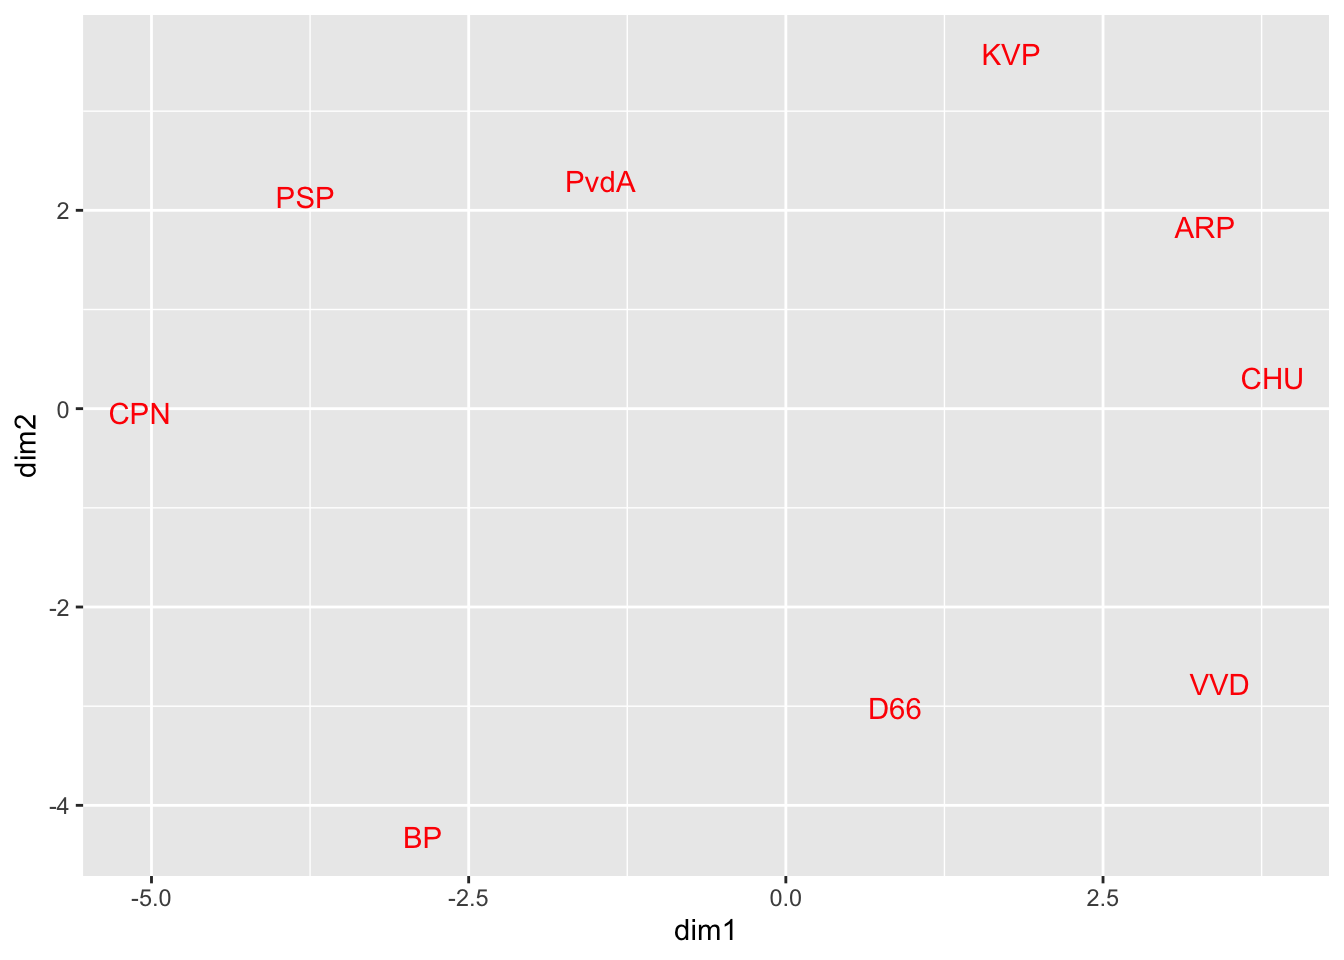
\includegraphics{av_files/figure-pdf/pxls-1.pdf}

}

\caption{Configuration Least Squares}

\end{figure}%

\begin{figure}[H]

{\centering 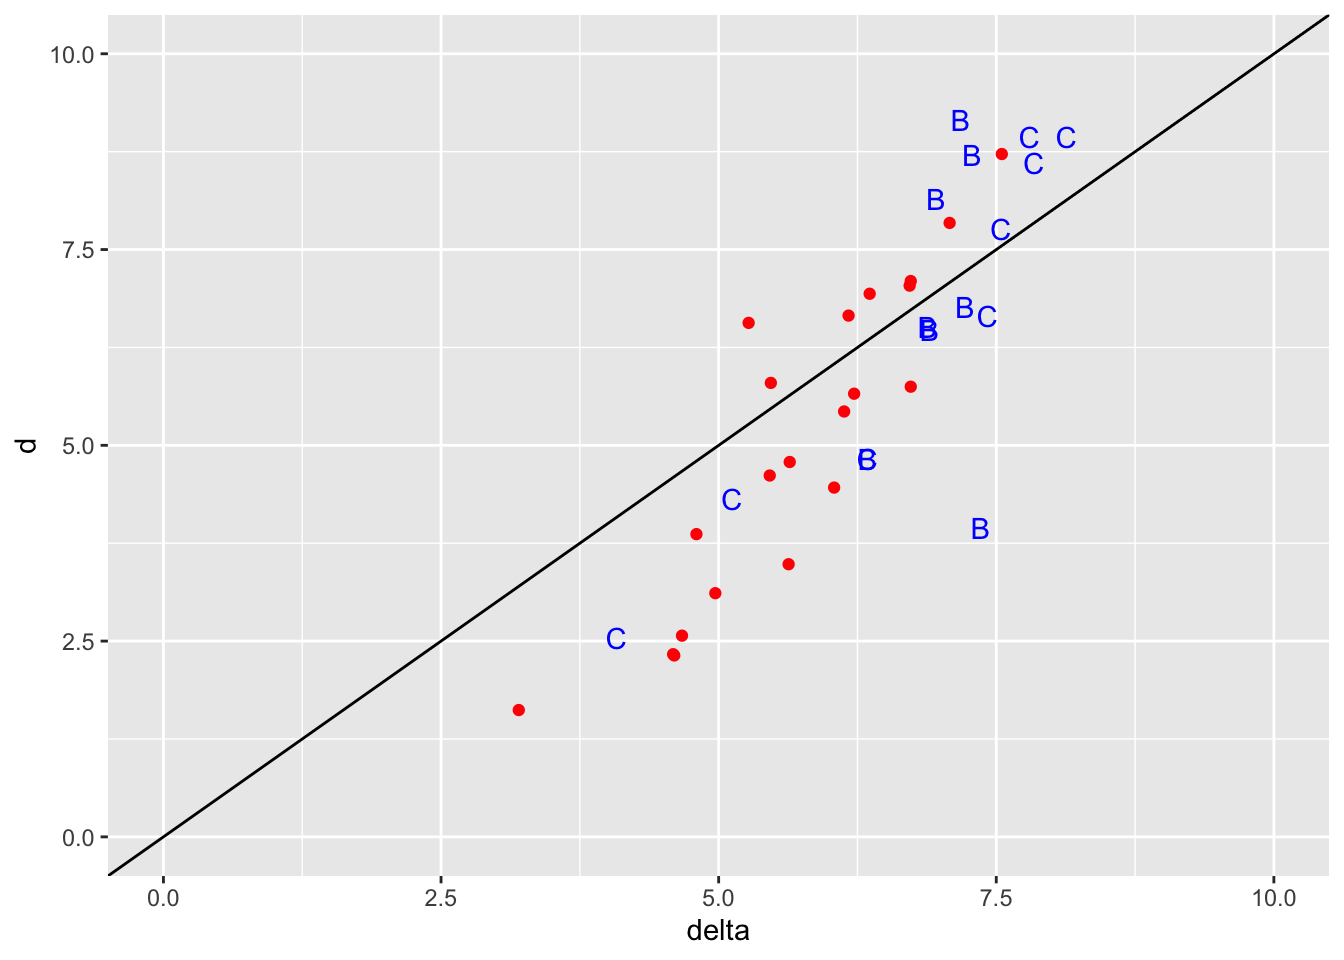
\includegraphics{av_files/figure-pdf/pdls-1.pdf}

}

\caption{Shepard Plot Least Squares}

\end{figure}%

\begin{figure}[H]

{\centering 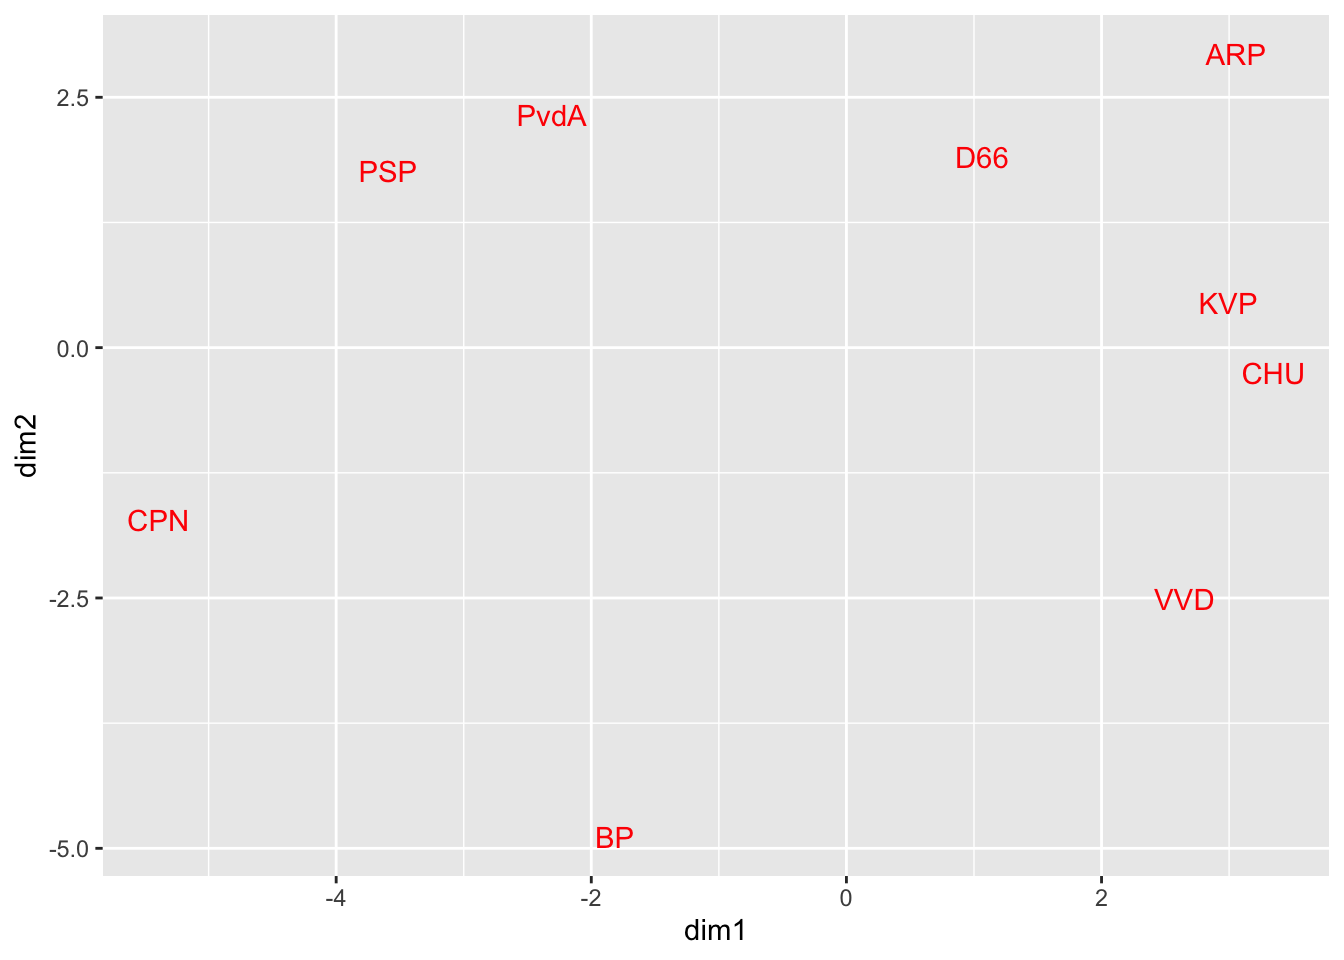
\includegraphics{av_files/figure-pdf/pxav-1.pdf}

}

\caption{Configuration Least Absolute Value}

\end{figure}%

\begin{figure}[H]

{\centering 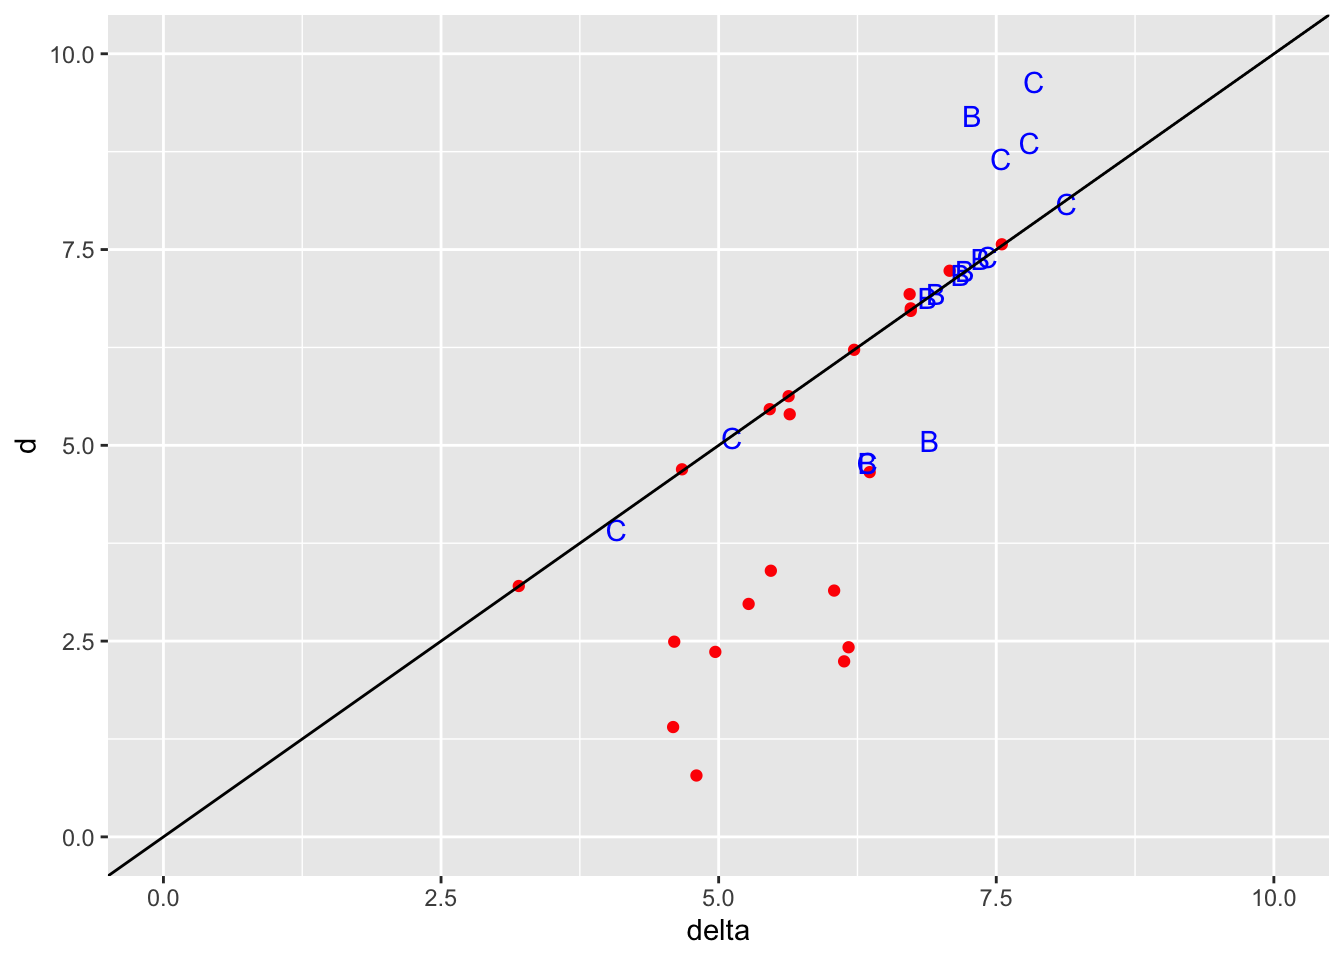
\includegraphics{av_files/figure-pdf/pdav-1.pdf}

}

\caption{Shepard Plot Least Absolute Value}

\end{figure}%

\begin{figure}[H]

{\centering \includegraphics{av_files/figure-pdf/pxhmed-1.pdf}

}

\caption{Configuration Median Huber}

\end{figure}%

\begin{figure}[H]

{\centering \includegraphics{av_files/figure-pdf/pdhmed-1.pdf}

}

\caption{Shepard Plot Median Huber}

\end{figure}%

\begin{figure}[H]

{\centering 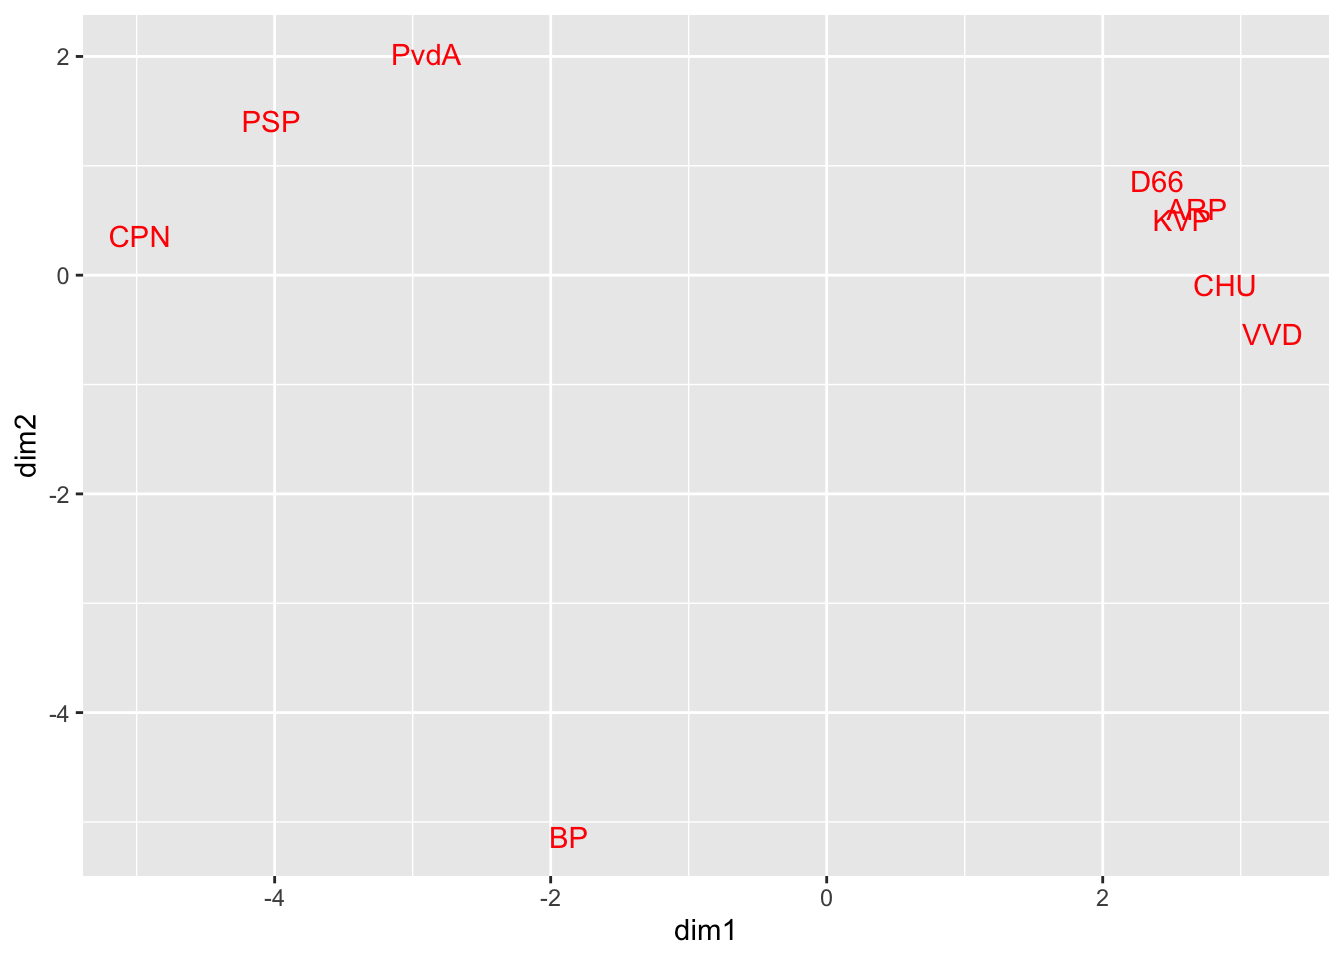
\includegraphics{av_files/figure-pdf/pxtmed-1.pdf}

}

\caption{Configuration Median Tukey}

\end{figure}%

\begin{figure}[H]

{\centering 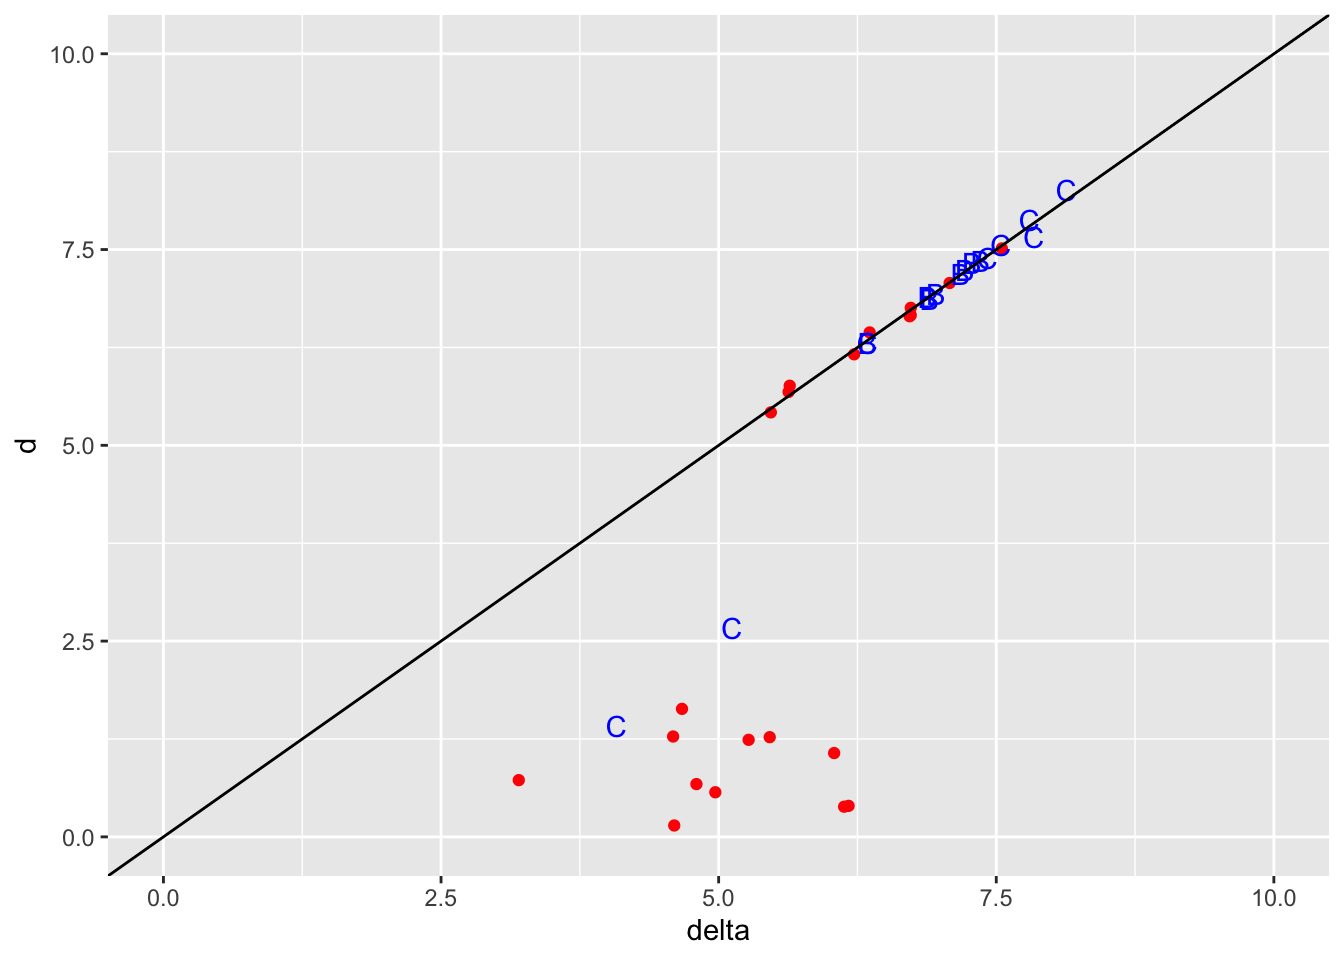
\includegraphics{av_files/figure-pdf/pdtmed-1.pdf}

}

\caption{Shepard Plot Median Tukey}

\end{figure}%

\section{Discussion}\label{discussion}

Fixed weights

Minimize \[
\sum w_k\ f(\delta_k-d_k(X))
\] if \(f''(x)\leq K\).

\[
f(\delta_k-d_k(X))\leq f(\delta_k-d_k(Y))+f'(\delta_k-d_k(Y))(d_k(Y)-d_k(X))+\frac12K(d_k(Y)-d_k(X))^2
\] Minimize \[
\left[d_k(X)-\{d_k(Y))-K^{-1}f'(\delta_k-d_k(Y))\}\right]^2
\]

\section{Code}\label{code}

The function smacofRobust has a parameter ``engine'', which can be equal
to smacofAV, smacofHuber, smacofTukey, or smacofConvolution. These four
small modules compute the respective loss function values and weights
for the IRLS procedure. This makes it easy to add additional robust loss
functions.

\begin{Shaded}
\begin{Highlighting}[]
\NormalTok{smacofRobust }\OtherTok{\textless{}{-}} \ControlFlowTok{function}\NormalTok{(delta,}
                         \AttributeTok{weights =} \DecValTok{1} \SpecialCharTok{{-}} \FunctionTok{diag}\NormalTok{(}\FunctionTok{nrow}\NormalTok{(delta)),}
                         \AttributeTok{ndim =} \DecValTok{2}\NormalTok{,}
                         \AttributeTok{xold =} \FunctionTok{smacofTorgerson}\NormalTok{(delta, ndim),}
                         \AttributeTok{engine =}\NormalTok{ smacofAV,}
                         \AttributeTok{cons =} \DecValTok{0}\NormalTok{,}
                         \AttributeTok{itmax =} \DecValTok{1000}\NormalTok{,}
                         \AttributeTok{eps =} \FloatTok{1e{-}15}\NormalTok{,}
                         \AttributeTok{verbose =} \ConstantTok{TRUE}\NormalTok{) \{}
\NormalTok{  nobj }\OtherTok{\textless{}{-}} \FunctionTok{nrow}\NormalTok{(delta)}
\NormalTok{  wmax }\OtherTok{\textless{}{-}} \FunctionTok{max}\NormalTok{(weights)}
\NormalTok{  dold }\OtherTok{\textless{}{-}} \FunctionTok{as.matrix}\NormalTok{(}\FunctionTok{dist}\NormalTok{(xold))}
\NormalTok{  h }\OtherTok{\textless{}{-}} \FunctionTok{engine}\NormalTok{(nobj, weights, delta, dold, cons)}
\NormalTok{  rold }\OtherTok{\textless{}{-}}\NormalTok{ h}\SpecialCharTok{$}\NormalTok{resi}
\NormalTok{  wold }\OtherTok{\textless{}{-}}\NormalTok{ h}\SpecialCharTok{$}\NormalTok{wght}
\NormalTok{  sold }\OtherTok{\textless{}{-}}\NormalTok{ h}\SpecialCharTok{$}\NormalTok{strs}
\NormalTok{  itel }\OtherTok{\textless{}{-}} \DecValTok{1}
  \ControlFlowTok{repeat}\NormalTok{ \{}
\NormalTok{    vmat }\OtherTok{\textless{}{-}} \SpecialCharTok{{-}}\NormalTok{wold}
    \FunctionTok{diag}\NormalTok{(vmat) }\OtherTok{\textless{}{-}} \SpecialCharTok{{-}}\FunctionTok{rowSums}\NormalTok{(vmat)}
\NormalTok{    vinv }\OtherTok{\textless{}{-}} \FunctionTok{solve}\NormalTok{(vmat }\SpecialCharTok{+}\NormalTok{ (}\DecValTok{1} \SpecialCharTok{/}\NormalTok{ nobj)) }\SpecialCharTok{{-}}\NormalTok{ (}\DecValTok{1} \SpecialCharTok{/}\NormalTok{ nobj)}
\NormalTok{    bmat }\OtherTok{\textless{}{-}} \SpecialCharTok{{-}}\NormalTok{wold }\SpecialCharTok{*}\NormalTok{ delta }\SpecialCharTok{/}\NormalTok{ (dold }\SpecialCharTok{+} \FunctionTok{diag}\NormalTok{(nobj))}
    \FunctionTok{diag}\NormalTok{(bmat) }\OtherTok{\textless{}{-}} \SpecialCharTok{{-}}\FunctionTok{rowSums}\NormalTok{(bmat)}
\NormalTok{    xnew }\OtherTok{\textless{}{-}}\NormalTok{ vinv }\SpecialCharTok{\%*\%}\NormalTok{ (bmat }\SpecialCharTok{\%*\%}\NormalTok{ xold)}
\NormalTok{    dnew }\OtherTok{\textless{}{-}} \FunctionTok{as.matrix}\NormalTok{(}\FunctionTok{dist}\NormalTok{(xnew))}
\NormalTok{    h }\OtherTok{\textless{}{-}} \FunctionTok{engine}\NormalTok{(nobj, weights, delta, dnew, cons)}
\NormalTok{    rnew }\OtherTok{\textless{}{-}}\NormalTok{ h}\SpecialCharTok{$}\NormalTok{resi}
\NormalTok{    wnew }\OtherTok{\textless{}{-}}\NormalTok{ h}\SpecialCharTok{$}\NormalTok{wght}
\NormalTok{    snew }\OtherTok{\textless{}{-}}\NormalTok{ h}\SpecialCharTok{$}\NormalTok{strs}
    \ControlFlowTok{if}\NormalTok{ (verbose) \{}
      \FunctionTok{cat}\NormalTok{(}
        \StringTok{"itel "}\NormalTok{,}
        \FunctionTok{formatC}\NormalTok{(itel, }\AttributeTok{width =} \DecValTok{4}\NormalTok{, }\AttributeTok{format =} \StringTok{"d"}\NormalTok{),}
        \StringTok{"sold "}\NormalTok{,}
        \FunctionTok{formatC}\NormalTok{(sold, }\AttributeTok{digits =} \DecValTok{10}\NormalTok{, }\AttributeTok{format =} \StringTok{"f"}\NormalTok{),}
        \StringTok{"snew "}\NormalTok{,}
        \FunctionTok{formatC}\NormalTok{(snew, }\AttributeTok{digits =} \DecValTok{10}\NormalTok{, }\AttributeTok{format =} \StringTok{"f"}\NormalTok{),}
        \StringTok{"}\SpecialCharTok{\textbackslash{}n}\StringTok{"}
\NormalTok{      )}
\NormalTok{    \}}
    \ControlFlowTok{if}\NormalTok{ ((itel }\SpecialCharTok{==}\NormalTok{ itmax) }\SpecialCharTok{||}\NormalTok{ ((sold }\SpecialCharTok{{-}}\NormalTok{ snew) }\SpecialCharTok{\textless{}}\NormalTok{ eps)) \{}
      \ControlFlowTok{break}
\NormalTok{    \}}
\NormalTok{    xold }\OtherTok{\textless{}{-}}\NormalTok{ xnew}
\NormalTok{    dold }\OtherTok{\textless{}{-}}\NormalTok{ dnew}
\NormalTok{    sold }\OtherTok{\textless{}{-}}\NormalTok{ snew}
\NormalTok{    wold }\OtherTok{\textless{}{-}}\NormalTok{ wnew}
\NormalTok{    rold }\OtherTok{\textless{}{-}}\NormalTok{ rnew}
\NormalTok{    itel }\OtherTok{\textless{}{-}}\NormalTok{ itel }\SpecialCharTok{+} \DecValTok{1}
\NormalTok{  \}}
  \FunctionTok{return}\NormalTok{(}\FunctionTok{list}\NormalTok{(}
    \AttributeTok{x =}\NormalTok{ xnew,}
    \AttributeTok{s =}\NormalTok{ snew,}
    \AttributeTok{d =}\NormalTok{ dnew,}
    \AttributeTok{r =}\NormalTok{ rnew,}
    \AttributeTok{itel =}\NormalTok{ itel}
\NormalTok{  ))}
\NormalTok{\}}

\NormalTok{smacofTorgerson }\OtherTok{\textless{}{-}} \ControlFlowTok{function}\NormalTok{(delta, ndim) \{}
\NormalTok{  dd }\OtherTok{\textless{}{-}}\NormalTok{ delta }\SpecialCharTok{\^{}} \DecValTok{2}
\NormalTok{  rd }\OtherTok{\textless{}{-}} \FunctionTok{apply}\NormalTok{(dd, }\DecValTok{1}\NormalTok{, mean)}
\NormalTok{  md }\OtherTok{\textless{}{-}} \FunctionTok{mean}\NormalTok{(dd)}
\NormalTok{  sd }\OtherTok{\textless{}{-}} \SpecialCharTok{{-}}\NormalTok{.}\DecValTok{5} \SpecialCharTok{*}\NormalTok{ (dd }\SpecialCharTok{{-}} \FunctionTok{outer}\NormalTok{(rd, rd, }\StringTok{"+"}\NormalTok{) }\SpecialCharTok{+}\NormalTok{ md)}
\NormalTok{  ed }\OtherTok{\textless{}{-}} \FunctionTok{eigen}\NormalTok{(sd)}
  \FunctionTok{return}\NormalTok{(ed}\SpecialCharTok{$}\NormalTok{vectors[, }\DecValTok{1}\SpecialCharTok{:}\NormalTok{ndim] }\SpecialCharTok{\%*\%} \FunctionTok{diag}\NormalTok{(}\FunctionTok{sqrt}\NormalTok{(ed}\SpecialCharTok{$}\NormalTok{values[}\DecValTok{1}\SpecialCharTok{:}\NormalTok{ndim])))}
\NormalTok{\}}

\NormalTok{smacofAV }\OtherTok{\textless{}{-}} \ControlFlowTok{function}\NormalTok{(nobj, wmat, delta, dmat, cons) \{}
\NormalTok{  resi }\OtherTok{\textless{}{-}} \FunctionTok{sqrt}\NormalTok{((delta }\SpecialCharTok{{-}}\NormalTok{ dmat) }\SpecialCharTok{\^{}} \DecValTok{2} \SpecialCharTok{+}\NormalTok{ cons)}
\NormalTok{  resi }\OtherTok{\textless{}{-}} \FunctionTok{ifelse}\NormalTok{(resi }\SpecialCharTok{\textless{}} \FloatTok{1e{-}10}\NormalTok{, }\DecValTok{2} \SpecialCharTok{*} \FunctionTok{max}\NormalTok{(wmat), resi)}
\NormalTok{  rmin }\OtherTok{\textless{}{-}} \FunctionTok{sqrt}\NormalTok{(cons)}
\NormalTok{  wght }\OtherTok{\textless{}{-}}\NormalTok{ wmat }\SpecialCharTok{/}\NormalTok{ (resi }\SpecialCharTok{+} \FunctionTok{diag}\NormalTok{(nobj))}
\NormalTok{  strs }\OtherTok{\textless{}{-}} \FunctionTok{sum}\NormalTok{(wmat }\SpecialCharTok{*}\NormalTok{ resi) }\SpecialCharTok{{-}}\NormalTok{ rmin }\SpecialCharTok{*} \FunctionTok{sum}\NormalTok{(wmat)}
  \FunctionTok{return}\NormalTok{(}\FunctionTok{list}\NormalTok{(}\AttributeTok{resi =}\NormalTok{ resi, }\AttributeTok{wght =}\NormalTok{ wght, }\AttributeTok{strs =}\NormalTok{ strs))}
\NormalTok{\}}

\NormalTok{smacofLP }\OtherTok{\textless{}{-}} \ControlFlowTok{function}\NormalTok{(nobj, wmat, delta, dmat, cons) \{}
\NormalTok{  resi }\OtherTok{\textless{}{-}}\NormalTok{ ((delta }\SpecialCharTok{{-}}\NormalTok{ dmat) }\SpecialCharTok{\^{}} \DecValTok{2} \SpecialCharTok{+}\NormalTok{ cons[}\DecValTok{1}\NormalTok{]) }\SpecialCharTok{\^{}}\NormalTok{ cons[}\DecValTok{2}\NormalTok{]}
\NormalTok{  rmin }\OtherTok{\textless{}{-}}\NormalTok{ cons[}\DecValTok{1}\NormalTok{] }\SpecialCharTok{\^{}}\NormalTok{ cons[}\DecValTok{2}\NormalTok{]}
\NormalTok{  wght }\OtherTok{\textless{}{-}}\NormalTok{ wmat }\SpecialCharTok{*}\NormalTok{ ((delta }\SpecialCharTok{{-}}\NormalTok{ dmat) }\SpecialCharTok{\^{}} \DecValTok{2} \SpecialCharTok{+}\NormalTok{ cons[}\DecValTok{1}\NormalTok{] }\SpecialCharTok{+} \FunctionTok{diag}\NormalTok{(nobj)) }\SpecialCharTok{\^{}}\NormalTok{ (cons[}\DecValTok{2}\NormalTok{] }\SpecialCharTok{{-}} \DecValTok{1}\NormalTok{)}
\NormalTok{  strs }\OtherTok{\textless{}{-}} \FunctionTok{sum}\NormalTok{(wmat }\SpecialCharTok{*}\NormalTok{ resi) }\SpecialCharTok{{-}}\NormalTok{ rmin }\SpecialCharTok{*} \FunctionTok{sum}\NormalTok{(wmat)}
  \FunctionTok{return}\NormalTok{(}\FunctionTok{list}\NormalTok{(}\AttributeTok{resi =}\NormalTok{ resi, }\AttributeTok{wght =}\NormalTok{ wght, }\AttributeTok{strs =}\NormalTok{ strs))}
\NormalTok{\}}

\NormalTok{smacofConvolution }\OtherTok{\textless{}{-}} \ControlFlowTok{function}\NormalTok{(nobj, wmat, delta, dmat, cons) \{}
\NormalTok{  difi }\OtherTok{\textless{}{-}}\NormalTok{ delta }\SpecialCharTok{{-}}\NormalTok{ dmat}
\NormalTok{  resi }\OtherTok{\textless{}{-}}\NormalTok{ difi }\SpecialCharTok{*}\NormalTok{ (}\DecValTok{2} \SpecialCharTok{*} \FunctionTok{pnorm}\NormalTok{(difi }\SpecialCharTok{/}\NormalTok{ cons) }\SpecialCharTok{{-}} \DecValTok{1}\NormalTok{) }\SpecialCharTok{+} \DecValTok{2} \SpecialCharTok{*}\NormalTok{ cons }\SpecialCharTok{*} \FunctionTok{dnorm}\NormalTok{(difi }\SpecialCharTok{/}\NormalTok{ cons)}
\NormalTok{  rmin }\OtherTok{\textless{}{-}} \DecValTok{2} \SpecialCharTok{*}\NormalTok{ cons }\SpecialCharTok{*} \FunctionTok{dnorm}\NormalTok{(}\DecValTok{0}\NormalTok{)}
\NormalTok{  wght }\OtherTok{\textless{}{-}}\NormalTok{ wmat }\SpecialCharTok{*}\NormalTok{ (}\FunctionTok{pnorm}\NormalTok{(difi }\SpecialCharTok{/}\NormalTok{ cons) }\SpecialCharTok{{-}} \FloatTok{0.5}\NormalTok{) }\SpecialCharTok{/}\NormalTok{ (difi }\SpecialCharTok{+} \FunctionTok{diag}\NormalTok{(nobj))}
\NormalTok{  strs }\OtherTok{\textless{}{-}} \FunctionTok{sum}\NormalTok{(wmat }\SpecialCharTok{*}\NormalTok{ resi) }\SpecialCharTok{{-}}\NormalTok{ rmin }\SpecialCharTok{*} \FunctionTok{sum}\NormalTok{(wmat)}
  \FunctionTok{return}\NormalTok{(}\FunctionTok{list}\NormalTok{(}\AttributeTok{resi =}\NormalTok{ resi, }\AttributeTok{wght =}\NormalTok{ wght, }\AttributeTok{strs =}\NormalTok{ strs))}
\NormalTok{\}}

\NormalTok{smacofHuber }\OtherTok{\textless{}{-}} \ControlFlowTok{function}\NormalTok{(nobj, wmat, delta, dmat, cons) \{}
\NormalTok{  difi }\OtherTok{\textless{}{-}}\NormalTok{ delta }\SpecialCharTok{{-}}\NormalTok{ dmat}
\NormalTok{  resi }\OtherTok{\textless{}{-}} \FunctionTok{ifelse}\NormalTok{(}\FunctionTok{abs}\NormalTok{(difi) }\SpecialCharTok{\textless{}}\NormalTok{ cons, (difi }\SpecialCharTok{\^{}} \DecValTok{2}\NormalTok{) }\SpecialCharTok{/} \DecValTok{2}\NormalTok{, cons }\SpecialCharTok{*} \FunctionTok{abs}\NormalTok{(difi) }\SpecialCharTok{{-}}\NormalTok{ ((cons }\SpecialCharTok{\^{}} \DecValTok{2}\NormalTok{) }\SpecialCharTok{/} \DecValTok{2}\NormalTok{))}
\NormalTok{  wght }\OtherTok{\textless{}{-}} \FunctionTok{ifelse}\NormalTok{(}\FunctionTok{abs}\NormalTok{(difi) }\SpecialCharTok{\textless{}}\NormalTok{ cons, wmat,}
\NormalTok{                 wmat }\SpecialCharTok{*} \FunctionTok{sign}\NormalTok{(difi }\SpecialCharTok{{-}}\NormalTok{ cons) }\SpecialCharTok{*}\NormalTok{ cons }\SpecialCharTok{/}\NormalTok{ (difi }\SpecialCharTok{+} \FunctionTok{diag}\NormalTok{(nobj)))}
\NormalTok{  strs }\OtherTok{\textless{}{-}} \FunctionTok{sum}\NormalTok{(wmat }\SpecialCharTok{*}\NormalTok{ resi)}
  \FunctionTok{return}\NormalTok{(}\FunctionTok{list}\NormalTok{(}\AttributeTok{resi =}\NormalTok{ resi, }\AttributeTok{wght =}\NormalTok{ wght, }\AttributeTok{strs =}\NormalTok{ strs))}
\NormalTok{\}}

\NormalTok{smacofTukey }\OtherTok{\textless{}{-}} \ControlFlowTok{function}\NormalTok{(nobj, wmat, delta, dmat, cons) \{}
\NormalTok{  cans }\OtherTok{\textless{}{-}}\NormalTok{ (cons }\SpecialCharTok{\^{}} \DecValTok{2}\NormalTok{) }\SpecialCharTok{/} \DecValTok{6}
\NormalTok{  difi }\OtherTok{\textless{}{-}}\NormalTok{ delta }\SpecialCharTok{{-}}\NormalTok{ dmat}
\NormalTok{  resi }\OtherTok{\textless{}{-}} \FunctionTok{ifelse}\NormalTok{(}\FunctionTok{abs}\NormalTok{(difi) }\SpecialCharTok{\textless{}}\NormalTok{ cons,}
\NormalTok{                 cans }\SpecialCharTok{*}\NormalTok{ (}\DecValTok{1} \SpecialCharTok{{-}}\NormalTok{ (}\DecValTok{1} \SpecialCharTok{{-}}\NormalTok{ (difi }\SpecialCharTok{/}\NormalTok{ cons) }\SpecialCharTok{\^{}} \DecValTok{2}\NormalTok{) }\SpecialCharTok{\^{}} \DecValTok{3}\NormalTok{), cans)}
\NormalTok{  wght }\OtherTok{\textless{}{-}}\NormalTok{ wmat }\SpecialCharTok{*} \FunctionTok{ifelse}\NormalTok{(}\FunctionTok{abs}\NormalTok{(difi) }\SpecialCharTok{\textless{}}\NormalTok{ cons,}
\NormalTok{                 (}\DecValTok{1} \SpecialCharTok{{-}}\NormalTok{ (difi }\SpecialCharTok{/}\NormalTok{ cons) }\SpecialCharTok{\^{}} \DecValTok{2}\NormalTok{) }\SpecialCharTok{\^{}} \DecValTok{2}\NormalTok{, }\DecValTok{0}\NormalTok{)}
\NormalTok{  strs }\OtherTok{\textless{}{-}} \FunctionTok{sum}\NormalTok{(wmat }\SpecialCharTok{*}\NormalTok{ resi)}
  \FunctionTok{return}\NormalTok{(}\FunctionTok{list}\NormalTok{(}\AttributeTok{resi =}\NormalTok{ resi, }\AttributeTok{wght =}\NormalTok{ wght, }\AttributeTok{strs =}\NormalTok{ strs))}
\NormalTok{\}}

\NormalTok{smacofCauchy }\OtherTok{\textless{}{-}} \ControlFlowTok{function}\NormalTok{(nobj, wmat, delta, dmat, cons) \{}
\NormalTok{  difi }\OtherTok{\textless{}{-}}\NormalTok{ delta }\SpecialCharTok{{-}}\NormalTok{ dmat}
\NormalTok{  resi }\OtherTok{\textless{}{-}} \FunctionTok{log}\NormalTok{((difi }\SpecialCharTok{/}\NormalTok{ cons) }\SpecialCharTok{\^{}} \DecValTok{2} \SpecialCharTok{+} \DecValTok{1}\NormalTok{)}
\NormalTok{  wght }\OtherTok{\textless{}{-}}\NormalTok{ wmat }\SpecialCharTok{*}\NormalTok{ (}\DecValTok{1} \SpecialCharTok{/}\NormalTok{ ((difi }\SpecialCharTok{/}\NormalTok{ cons) }\SpecialCharTok{\^{}} \DecValTok{2} \SpecialCharTok{+} \DecValTok{1}\NormalTok{))}
\NormalTok{  strs }\OtherTok{\textless{}{-}} \FunctionTok{sum}\NormalTok{(wmat }\SpecialCharTok{*}\NormalTok{ resi)}
  \FunctionTok{return}\NormalTok{(}\FunctionTok{list}\NormalTok{(}\AttributeTok{resi =}\NormalTok{ resi, }\AttributeTok{wght =}\NormalTok{ wght, }\AttributeTok{strs =}\NormalTok{ strs))}
\NormalTok{\}}

\NormalTok{smacofWelsch }\OtherTok{\textless{}{-}} \ControlFlowTok{function}\NormalTok{(nobj, wmat, delta, dmat, cons) \{}
\NormalTok{  difi }\OtherTok{\textless{}{-}}\NormalTok{ delta }\SpecialCharTok{{-}}\NormalTok{ dmat}
\NormalTok{  resi }\OtherTok{\textless{}{-}} \DecValTok{1} \SpecialCharTok{{-}} \FunctionTok{exp}\NormalTok{(}\SpecialCharTok{{-}}\NormalTok{(difi }\SpecialCharTok{/}\NormalTok{ cons) }\SpecialCharTok{\^{}} \DecValTok{2}\NormalTok{)}
\NormalTok{  wght }\OtherTok{\textless{}{-}}\NormalTok{ wmat }\SpecialCharTok{*} \FunctionTok{exp}\NormalTok{(}\SpecialCharTok{{-}}\NormalTok{(difi }\SpecialCharTok{/}\NormalTok{ cons) }\SpecialCharTok{\^{}} \DecValTok{2}\NormalTok{)}
\NormalTok{  strs }\OtherTok{\textless{}{-}} \FunctionTok{sum}\NormalTok{(wmat }\SpecialCharTok{*}\NormalTok{ resi)}
  \FunctionTok{return}\NormalTok{(}\FunctionTok{list}\NormalTok{(}\AttributeTok{resi =}\NormalTok{ resi, }\AttributeTok{wght =}\NormalTok{ wght, }\AttributeTok{strs =}\NormalTok{ strs))}
\NormalTok{\}}
\end{Highlighting}
\end{Shaded}

\section*{References}\label{references}
\addcontentsline{toc}{section}{References}

\phantomsection\label{refs}
\begin{CSLReferences}{1}{0}
\bibitem[\citeproctext]{ref-aftab_hartley_15}
Aftab, K., and R. Hartley. n.d. {``Convergence of Iteratively
Re-Weighted Least Squares to Robust m-Estimators.''} In \emph{2015 IEEE
Winter Conference on Applications of Computer Vision,} 480--87.
\url{https://doi.org/10.1109/WACV.2015.70}.

\bibitem[\citeproctext]{ref-barron_19}
Barron, J. T. 2019. {``A General and Adaptive Robust Loss Function.''}
In \emph{Proceedings 2019 IEEE/CVF Conferehce on Computer Vision and
Pattern Recognition}, 4331--39.
\url{https://openaccess.thecvf.com/content_CVPR_2019/papers/Barron_A_General_and_Adaptive_Robust_Loss_Function_CVPR_2019_paper.pdf}.

\bibitem[\citeproctext]{ref-charbonnier_blanc-feraud_aubert_barlaud_94}
Charbonnier, P., L. Blanc-Feraud, G. Aubert, and M. Barlaud. 1994.
{``{Two deterministic half-quadratic regularization algorithms for
computed imaging}.''} \emph{Proceedings of 1st International Conference
on Image Processing} 2: 168--72.
\url{https://doi.org/10.1109/icip.1994.413553}.

\bibitem[\citeproctext]{ref-degruijter_67}
De Gruijter, D. N. M. 1967. {``{The Cognitive Structure of Dutch
Political Parties in 1966}.''} Report E019-67. Psychological Institute,
University of Leiden.

\bibitem[\citeproctext]{ref-deleeuw_A_84f}
De Leeuw, J. 1984. {``{Differentiability of Kruskal's Stress at a Local
Minimum}.''} \emph{Psychometrika} 49: 111--13.

\bibitem[\citeproctext]{ref-deleeuw_C_94c}
---------. 1994. {``{Block Relaxation Algorithms in Statistics}.''} In
\emph{Information Systems and Data Analysis}, edited by H. H. Bock, W.
Lenski, and M. M. Richter, 308--24. Berlin: Springer Verlag.
\url{https://jansweb.netlify.app/publication/deleeuw-c-94-c/deleeuw-c-94-c.pdf}.

\bibitem[\citeproctext]{ref-deleeuw_E_18f}
---------. 2018. {``{MM Algorithms for Smoothed Absolute Values}.''}
2018.
\url{https://jansweb.netlify.app/publication/deleeuw-e-18-f/deleeuw-e-18-f.pdf}.

\bibitem[\citeproctext]{ref-deleeuw_E_20b}
---------. 2020. {``{Least Squares Absolute Value Regression}.''} 2020.
\url{https://jansweb.netlify.app/publication/deleeuw-e-20-b/deleeuw-e-20-b.pdf}.

\bibitem[\citeproctext]{ref-deleeuw_lange_A_09}
De Leeuw, J., and K. Lange. 2009. {``Sharp Quadratic Majorization in One
Dimension.''} \emph{Computational Statistics and Data Analysis} 53:
2471--84.

\bibitem[\citeproctext]{ref-groenen_heiser_meulman_99}
Groenen, P. J. F., W. J. Heiser, and J. J. Meulman. 1999. {``{Global
Optimization in Least-Squares Multidimensional Scaling by Distance
Smoothing}.''} \emph{Journal of Classification} 16: 225--54.

\bibitem[\citeproctext]{ref-heiser_87}
Heiser, W. J. 1987. {``{Correspondence Analysis with Least Absolute
Residuals}.''} \emph{Computational Statistica and Data Analysis} 5:
337--56.

\bibitem[\citeproctext]{ref-heiser_88}
---------. 1988. {``{Multidimensional Scaling with Least Absolute
Residuals}.''} In \emph{Classification and Related Methods of Data
Analysis}, edited by H. H. Bock, 455--62. North-Holland Publishing Co.

\bibitem[\citeproctext]{ref-huber_64}
Huber, P. J. 1964. {``Robust Estimation of a Location Parameter.''}
\emph{Annals of Mathematical Statistics} 35 (1): 73--101.

\bibitem[\citeproctext]{ref-lange_16}
Lange, K. 2016. \emph{MM Optimization Algorithms}. SIAM.

\bibitem[\citeproctext]{ref-phillips_02}
Phillips, R. F. 2002. {``Least Absolute Deviations Estimation via the EM
Algorithm.''} \emph{Statistics and Computing} 12: 281--85.

\bibitem[\citeproctext]{ref-pliner_96}
Pliner, V. 1996. {``{Metric Unidimensional Scaling and Global
Optimization}.''} \emph{Journal of Classification} 13: 3--18.

\bibitem[\citeproctext]{ref-ramirez_sanchez_kreinovich_argaez_14}
Ramirez, C., R. Sanchez, V. Kreinovich, and M. Argaez. 2014.
{``{\(\sqrt{x^2+\mu}\) is the Most Computationally Efficient Smooth
Approximation to \vert{}x\vert{}}.''} \emph{Journal of Uncertain
Systems} 8: 205--10.

\bibitem[\citeproctext]{ref-schlossmacher_73}
Schlossmacher, E. J. 1973. {``An Iterative Technique for Absolute
Deviations Curve Ftting.''} \emph{Journal of the American Statistical
Association} 68: 857--59.

\bibitem[\citeproctext]{ref-voronin_ozkaya_yoshida_15}
Voronin, S., G. Ozkaya, and Y. Yoshida. n.d. {``{Convolution Based
Smooth Approximations to the Absolute Value Function with Application to
Non-smooth Regularization}.''}

\end{CSLReferences}




\end{document}
